\chapter{Realizace}

\section{Prostředí}

Popsané algoritmy jsme implementovali v jazyce C99 \cite{ISO:C99}. Implementace probíhala v operačním systému Lubuntu \cite{lubuntu}, v IDE Eclipse CDT \cite{cdt}. Zdrojový kód byl kompilován pomocí překladače GNU C \cite{gcc}, s optimalizačním přepínačem \texttt{--Ofast}.

K ladění chyb pro práci s pamětí jsme použili nástroj Valgrind \cite{valgrind} s přepínači \texttt{----leak--check=full ----show-reachable=yes}. Běžící program jsme krokovali pomocí nástroje GNU Debugger \cite{gdb}. Zdrojový kód pro ladění chyb byl kompilován s přepínači \texttt{--Wall --pedantic --Og --ggdb}.

%-----------------------------------------------------------------------------

\section{Design implementace}

Po různých formátech požadujeme stejné operace, proto v programu zavádíme abstraktní matici a jednoduchý objektově orientovaný model \cite{schreiner1994objektorientierte}, která formáty dědí z virtuální matice. Obrázek \ref{fig:uml} ukazuje jednoduchý návrh tříd v UML.
	
\begin{figure}[htb]
	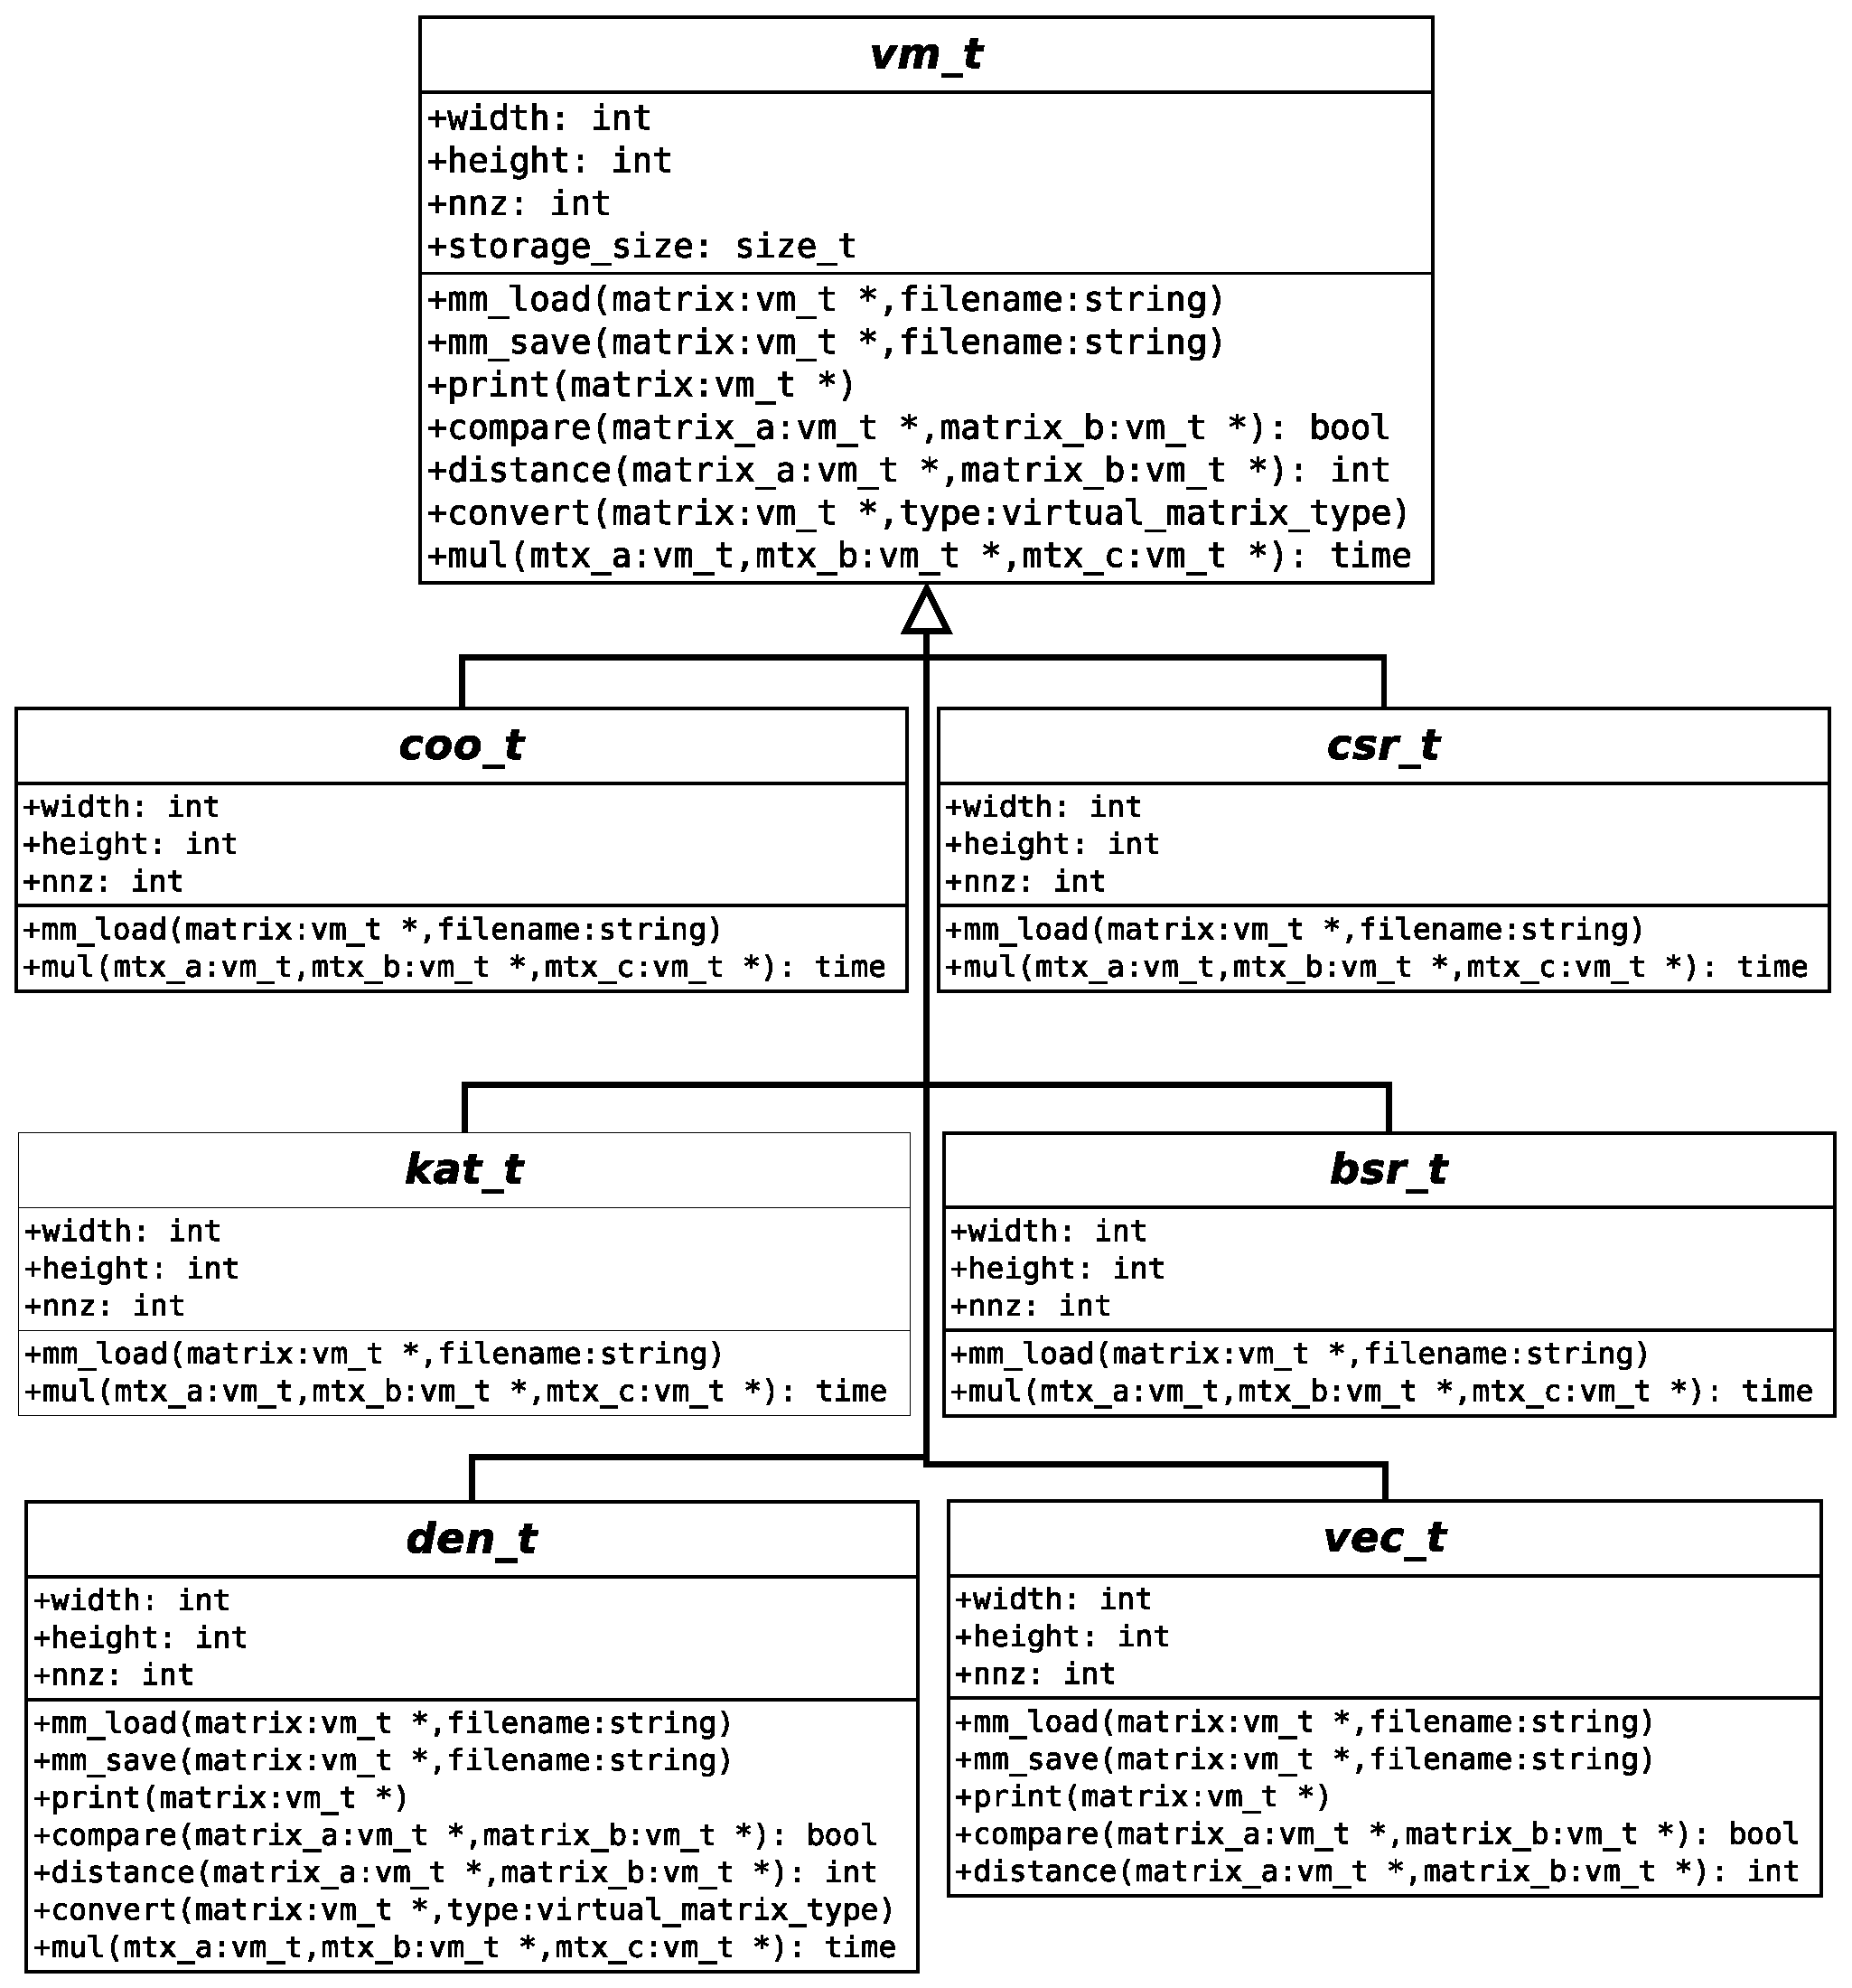
\includegraphics[width=1.0\textwidth]{./images/uml/uml}
	\caption{UML diagram tříd programu}
	\label{fig:uml}
\end{figure}

Program běží v příkazovém řádku bez GUI a je jednovláknový. Načte jednu nebo dvě matice v určitém formátu a vynásobí je. Pomocí přepínačů lze zobrazit nebo uložit výslednou matici, popřípadě vypsat některé údaje o načtených maticích. Podrobnější popis nastavení programu je v příloze.

%-----------------------------------------------------------------------------

\section{Implementace KAT}

U formátů COO, CSR, BSR je implementace přímočará podle pseudokódů. U implementace KAT máme více možností, proto zde popíšeme naší implementaci.

Jeden z důležitých parametrů je $k$, tedy maximální počet synů vnitřních uzlů. V naší implementaci je tento parametr uložen v konstantě \texttt{KAT.n}, pro připomenutí $KAT.n = sqrt(k)$. Překladač poté cykly, kde iterujeme do této konstanty, rozbalí. Překladači i explicitně sdělujeme, ať cykly rozbalí přes atribut \texttt{\_\_attribute\_\_((optimize("unroll-loops")))}.

V bakalářské práci Rozšíření implementace formátu kvadrantového stromu od Tomáše Karabely \cite{karabela} je Quadtree implementován jako strom, jehož listy tvoří virtuální matice podobným těm v naší práci. Protože jeho formát byl určený pro algoritmus LU rozklad, jeho virtuální matice musely umět přijímat i další prvky. Protože v naší práci se s formáty uložení řídké matice zachází jako s konstantami, rozhodli jsme se hodnoty prvků a informace v polích \texttt{row\_pointers} a \texttt{col\_indices} uložit mimo listy stromu. V listech se nachází ukazatel do velkého pole na příslušné místo pro daný list. Ušetříme tak práci knihovně libc s mnohonásobným volání funkce \texttt{malloc}.

\subsection{Tvoření stromu}

Při tvoření matice v KAT formátu pro každý prvek procházíme strom a hledáme správný list. Protože výška stromu je daná třemi parametry, tedy velikostí matice $n$, velikostí podmatice $sm\_size$ a počtem větvení uzlu $k$, nejefektivnější využití bude, pokud je $n$ bezezbytku dělitelné $k * sm\_size$. Pokud toto neplatí, rodiče listů budou mít část synů nevyužitých i při uložení husté matice. Protože se prvky do matice načítají po řádcích zleva doprava, je velká pravděpodobnost, že další načtený prvek bude patřit do stejného listu. Z tohoto důvodu si pamatujeme poslední list, a pokud prvek patří do něj, vrátíme jej. Algoritmus \ref{kat-create} ukazuje, jakým způsobem vyhledáváme list pro prvek.


\label{alg:kat-create}
\begin{algorithm}[htb]
	\caption{Vyhledání listu pro KAT matici}\label{kat-create}
	\begin{algorithmic}[1]
		\Procedure{KAT-getNode}{KAT, y, x}
		\If{ \{y, x\} $\in$ lastLeaf.area}
			\State \texttt{return lastLeaf;}
		\EndIf
		\State \texttt{tmpNode $\gets$ KAT.root;}
		\State \texttt{blockY $\gets$ 0;}\Comment{výřez matice}
		\State \texttt{blockX $\gets$ 0;}
		\State \texttt{blockS $\gets$ KAT.sm\_size;}
		\\\Comment{až do předposledního vnitřního uzlu traverzujeme podle velikosti KAT.n}
		\While{\texttt{blockS > (KAT.n * KAT.sm\_size)}}
			\State \texttt{nodeY $\gets$ (y - blockY) / (blockS / KAT.n);}
			\State \texttt{nodeX $\gets$ (x - blockX) / (blockS / KAT.n);}
			\State \texttt{tmpNode $\gets$ tmpNode.childs[nodeY][nodeX];}
			\State \texttt{blockY += nodeY * (blockS / KAT.n);}
			\State \texttt{blockX += nodeX * (blockS / KAT.n);}
			\State \texttt{blockS /= KAT.n;}
		\EndWhile
		\\\Comment{do posledního vnitnřního uzlu traverzujeme podle velikosti KAT.sm\_size}
		\State \texttt{nodeY $\gets$ (y - blockY) / KAT.sm\_size;}
		\State \texttt{nodeX $\gets$ (x - blockX) / KAT.sm\_size;}
		\State \texttt{tmpNode $\gets$ tmpNode.childs[nodeY][nodeX];} 	
		\\\Comment{nyní je tmpNode list}
		\State \texttt{tmpNode.y $\gets$ $\lfloor$y / KAT.sm\_size$\rfloor$ * KAT.sm\_size ;}
		\State \texttt{tmpNode.x $\gets$ $\lfloor$x / KAT.sm\_size$\rfloor$ * KAT.sm\_size ;}
		\State \texttt{lastLeaf $\gets$ tmpNode;}
		\State \texttt{return tmpNode;}
		\EndProcedure
	\end{algorithmic}
\end{algorithm}

\subsection{Násobení listů matice KAT}

Protože dovolujeme dva druhy listů, tedy hustý a řídký ve formátu CSR, bylo potřeba implementovat následující algoritmy:

\begin{enumerate}
  \item hustý list $\cdot$ hustý list
  \item hustý list $\cdot$ CSR list
  \item hustý list $\cdot$ vektor
  \item CSR list $\cdot$ hustý list
  \item CSR list $\cdot$ CSR list
  \item CSR list $\cdot$ vektor
\end{enumerate}

Protože tyto algoritmy jsou velice podobné již popsaným algoritmům \ref{algo}, ukážeme zde pouze násobení CSR listu s hustým listem.

\begin{algorithm}[htb]
	\caption{Násobení hustého KAT listu s CSR listem}\label{kat-mmm-den-csr}
	\begin{algorithmic}[1]
		\Procedure{KAT-MMM-DEN-CSR}{ka,kb,na,nb,c}\Comment{ka,kb=KAT matice; na,nb=listy, c = hustá matice}
		\For{\texttt{i $\gets$ 0 \TO ka.sm\_size}}
			\For{\texttt{j $\gets$ na.rp[i]\TO na.rp[i]}}
				\For{\texttt{k $\gets$ 0 \TO ka.sm\_size}}
					\State \texttt{C.v[na.y + i][nb.x + k] += na.v[j] * nb.v[ka.sm\_size * na.ci[j] + j];}
				\EndFor
			\EndFor
		\EndFor
		\EndProcedure
	\end{algorithmic}
\end{algorithm}


%-----------------------------------------------------------------------------

\section{Testování}

Pro ověření správnosti algoritmů je potřeba testovací software. Strategie testování v našem programu spočívá ve výběru testovacích matic, vynásobení v hustém formátu uložení, vynásobení v některém z řídkých formátů uložení a porovnání výsledků. Tento proces ukazuje algoritmus \ref{testing}.

\begin{algorithm}[htb]
	\caption{Testování}\label{testing}
	\begin{algorithmic}[1]
		\Procedure{\texttt{TestFormats}}{\texttt{PairList, FormatList}}
		\ForAll{\texttt{pair $\in$ PairList}}
				\State \texttt{denseA $\gets$ vm\_load(pair.a, DENSE);}
				\State \texttt{denseB $\gets$ vm\_load(pair.b, DENSE);}
				\State \texttt{denseC $\gets$ vm\_mul(denseA, denseB, denseC);}
			\ForAll{\texttt{format $\in$ FormatList}}		
				\State \texttt{sparseA $\gets$ vm\_load(pair.a, format);}
				\State \texttt{sparseB $\gets$ vm\_load(pair.b, format);}
				\State \texttt{sparseC $\gets$ vm\_mul(sparseA, sparseB, sparseC);}
				\If{ \texttt{vm\_compare(denseC, sparseC) = NOT\_SAME}}
					\State \texttt{print("Error:", pair.a, pair.b, format);}
				\EndIf
			\EndFor
		\EndFor
		\EndProcedure
	\end{algorithmic}
\end{algorithm}

Při testování jsme i na relativně malých maticích narazili na problém s numerickou stabilitou. Část z testovacích matic má velký desetinný rozvoj, a protože čísla jsou v různých formátech násobena v jiném pořadí, dochází k rozdílu mezi výsledky. Při kompilaci programu lze nastavit přesnost výpočtu pomocí typu proměnné pro uchování hodnot buď na \texttt{float}, \texttt{double} nebo \texttt{long double}. Při porovnávání dvou matic neporovnáváme hodnoty přímo, ale sledujeme velikost jejich rozdílu. V defaultní konfiguraci je povolená odchylka 0.001, při kompilaci ji lze změnit. Pokud spustíme testy  pouze s přesností \texttt{float}, část testů selže právě kvůli numerické stabilitě. 

%-----------------------------------------------------------------------------




\section{Měření}

Měření probíhalo na serveru \texttt{star.fit.cvut.cz}. Měřené parametry byly:
\begin{enumerate}
  \item Procentuální zrychlení výpočtu oproti formátu CSR
  \item Počet uzlů ve stromě KAT matice
  \item Velikost datových struktur matic
\end{enumerate}

V grafech značíme matici KAT jako $KAT.n kat block\_size$. Matici BSR jako $bsr block\_size$. 

Pro měření výsledků byly použity následující matice:

\begin{table}[H]
   \begin{tabular}{llllll}
    Skupina    & Název matice & Velikost & Nenulových prvků            & Oblast                  \\
    \hline
    GHS\_indef 	& exdata\_1 \cite{mtxexdata}    &  6001    & 2.269500 $\cdot 10^6$ & optimalizace \\
    Norris     	& heart1 \cite{mtxheart}       & 3557    & 1.385317 $\cdot 10^6$ & 2D/3D          \\
    Gupta     	& gupta3 \cite{mtxgupta}       &  16783    & 9323427 $\cdot 10^6$ & optimalizace         \\
    JGD\_SPG    	& EX6 \cite{mtxex}       & 6545     & 2.95680 $\cdot 10^5$ & kombinatorika \\
    MKS     		& fp \cite{mtxfp}       & 7548     & 8.34222 $\cdot 10^5$ & elektromagnetika         \\
    Belcastro   	& human-gene2 \cite{mtxhuman}        & 14340    & 1.8068388 $\cdot 10^7$ & graf         \\
    \end{tabular}
\end{table}

\subsection{Rychlost výpočtu}

Graf \ref{fig:mmmspeed} ukazuje zrychlení výpočtu na ukázkových maticích oproti násobení ve formátu CSR. Graf \ref{fig:mvmspeed} ukazuje stejný případ pro operaci násobení matice vektorem.

\begin{figure}[H]
	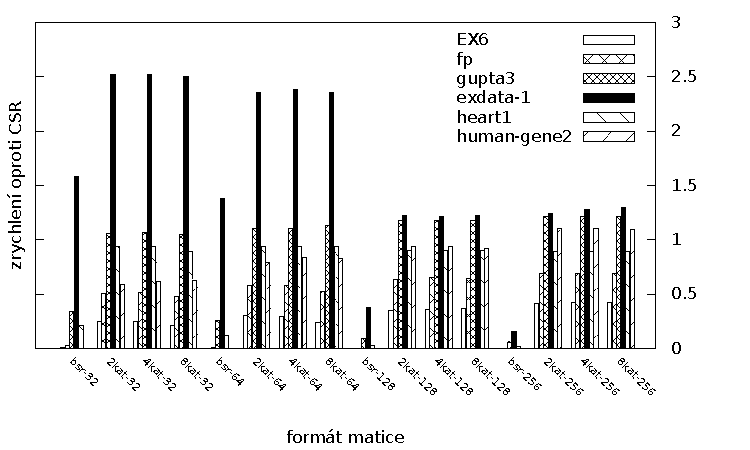
\includegraphics[width=1.0\textwidth]{./images/measure1/mmm-speedup}
	\caption{Zrychlení výpočtu matice $\cdot$ matice oproti formátu CSR}
	\label{fig:mmmspeed}
\end{figure}

\begin{figure}[H]
	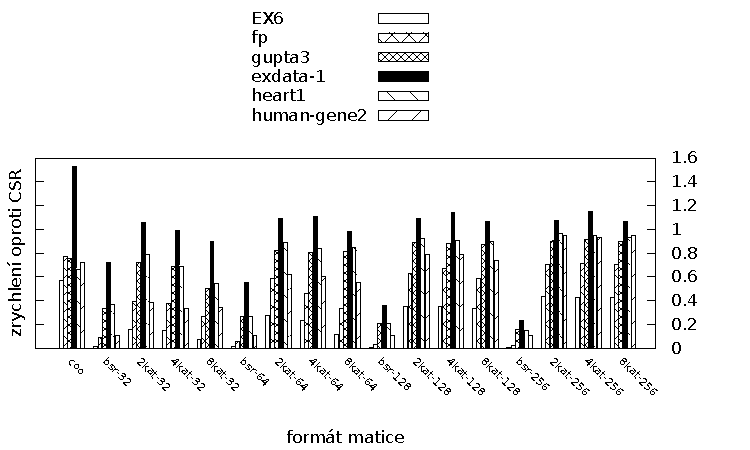
\includegraphics[width=1.0\textwidth]{./images/measure1/mvm-speedup}
	\caption{Zrychlení výpočtu matice $\cdot$ vektor oproti formátu CSR}
	\label{fig:mvmspeed}
\end{figure}

\subsection{Velikost datových struktur}

Graf \ref{fig:mtxsize} ukazuje v bytech přesnou velikost datových struktur matic v porovnání proti uložení matice v hustém formátu. Pro každý prvek bylo potřeba 8B dat, respektive prvky byly uloženy v proměnné typu double.

\begin{figure}[H]
	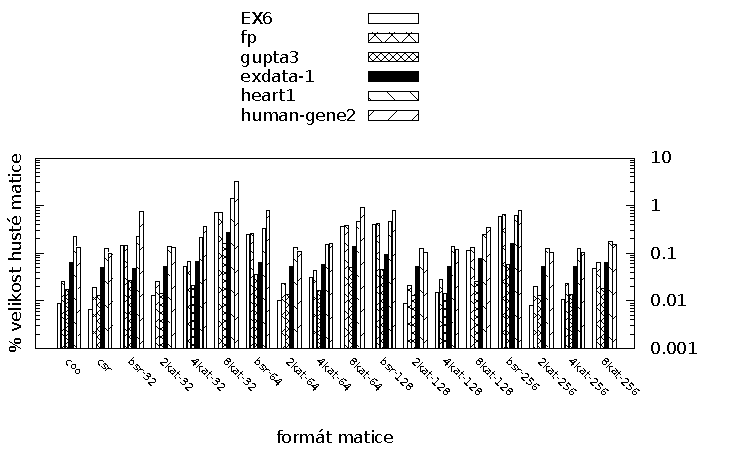
\includegraphics[width=1.0\textwidth]{./images/measure1/ram-up}
	\caption{Velikost datových struktur}
	\label{fig:mtxsize}
\end{figure}

\subsection{Počet uzlů v matici KAT}

Grafy \ref{fig:mtxsizeEX6} \ref{fig:mtxsizeexdata} \ref{fig:mtxsizefp} \ref{fig:mtxsizegupta} \ref{fig:mtxsizeheart} \ref{fig:mtxsizehuman} ukazují počet uzlů ve stromě a jejich druh.

\begin{figure}[htb]
	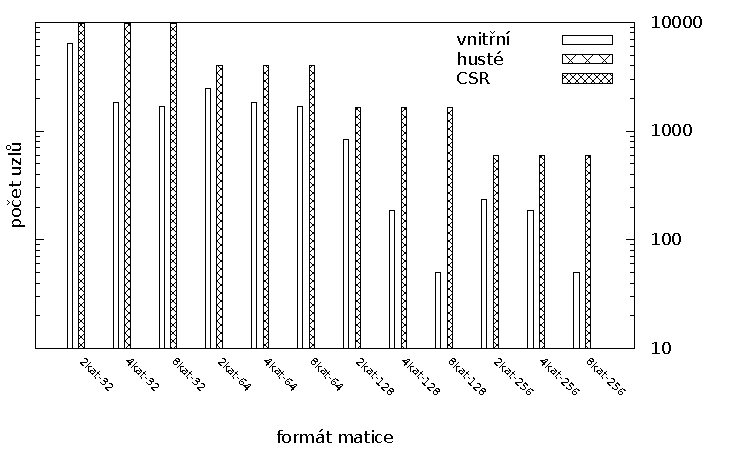
\includegraphics[width=1.0\textwidth]{./images/measure1/kat_nodes_EX6}
	\caption{Počet uzlů v matici KAT pro uložení matice EX6}
	\label{fig:mtxsizeEX6}
\end{figure}

\begin{figure}[htb]
	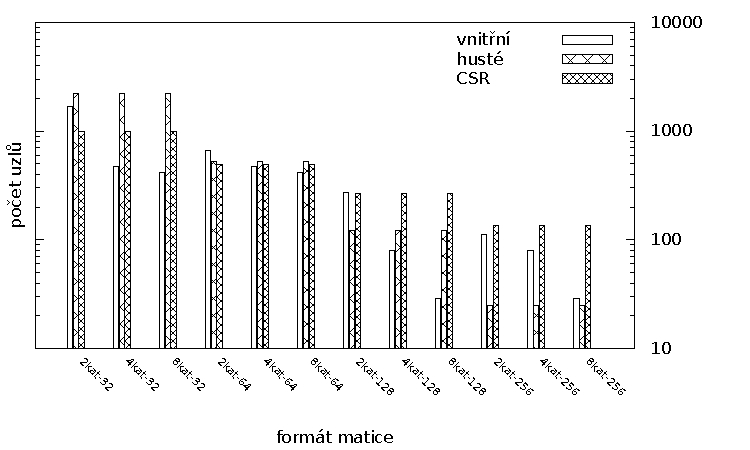
\includegraphics[width=1.0\textwidth]{./images/measure1/kat_nodes_exdata-1}
	\caption{Počet uzlů v matici KAT pro uložení matice exdata-1}
	\label{fig:mtxsizeexdata}
\end{figure}

\begin{figure}[htb]
	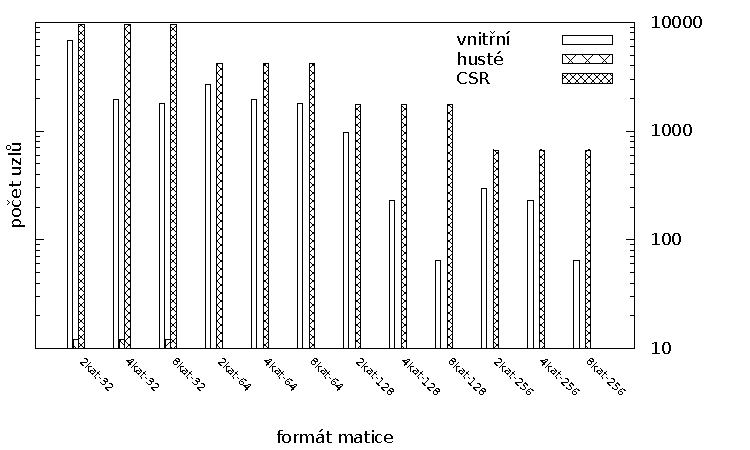
\includegraphics[width=1.0\textwidth]{./images/measure1/kat_nodes_fp}
	\caption{Počet uzlů v matici KAT pro uložení matice fp}
	\label{fig:mtxsizefp}
\end{figure}

\begin{figure}[htb]
	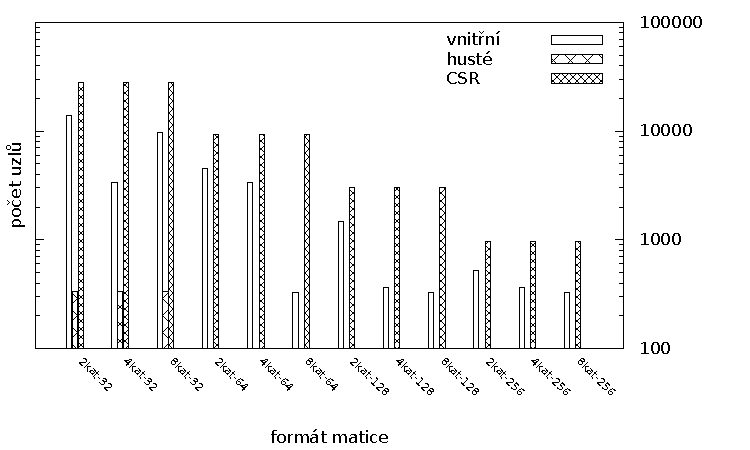
\includegraphics[width=1.0\textwidth]{./images/measure1/kat_nodes_gupta3}
	\caption{Počet uzlů v matici KAT pro uložení matice gupta3}
	\label{fig:mtxsizegupta}
\end{figure}

\begin{figure}[htb]
	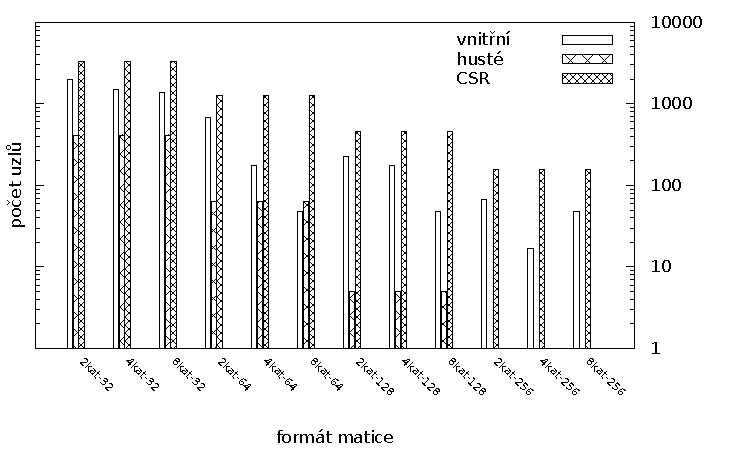
\includegraphics[width=1.0\textwidth]{./images/measure1/kat_nodes_heart1}
	\caption{Počet uzlů v matici KAT pro uložení matice heart1}
	\label{fig:mtxsizeheart}
\end{figure}

\begin{figure}[htb]
	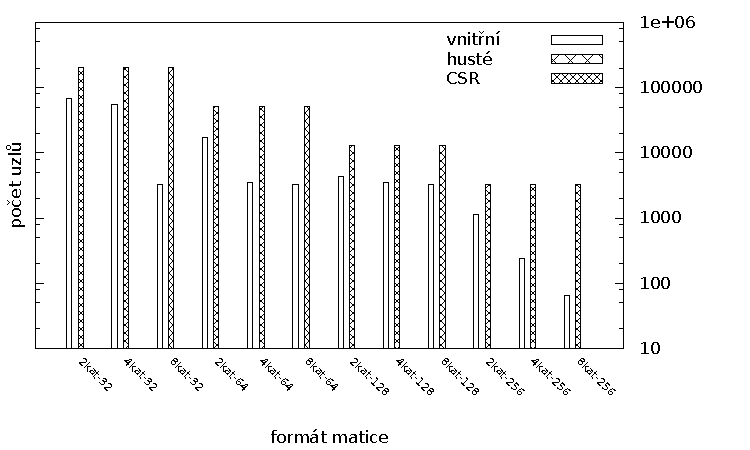
\includegraphics[width=1.0\textwidth]{./images/measure1/kat_nodes_human-gene2}
	\caption{Počet uzlů v matici KAT pro uložení matice human-gene2}
	\label{fig:mtxsizehuman}
\end{figure}


% \begin{sidewaysfigure}
% \end{sidewaysfigure}

\section{Porovnání výkonnosti s předpoklady}

Protože při násobení řídkých matic velmi záleží na rozložení jejich prvků, tak abychom porovnali teoretické předpoklady s naměřenými hodnotami, provedeme měření na hustých maticích o velikosti 256, 512, 1024 a 2048. Protože jsme použili pouze základní algoritmy  násobení, časová složitost by měla být \bigO$(n^3)$ pro násobení matice s maticí a \bigO$(n^2)$ pro násobení matice s vektorem. Paměťová složitost by měla být nejmenší u CSR a BSR, kde ukládáme u prvků pouze jejich hodnoty a sloupce. U formátu KAT by měla být paměťová složitost velká z důvodu ukládání struktury stromu.

\begin{figure}[htb]
	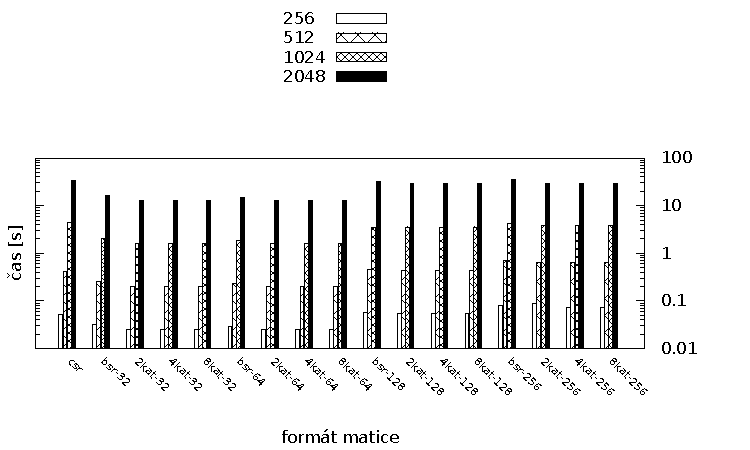
\includegraphics[width=1.0\textwidth]{./images/dense/mmm-speedtime}
	\caption{Čas násobení husté matice s hustou maticí v řídkém formátu}
	\label{fig:denmmm}
\end{figure}

\begin{figure}[htb]
	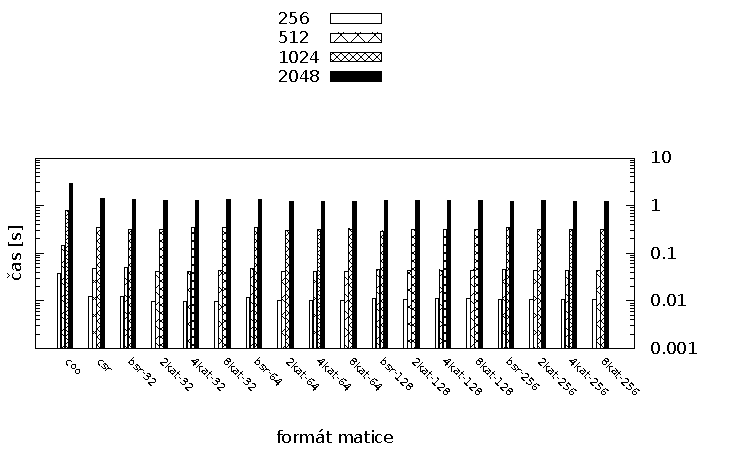
\includegraphics[width=1.0\textwidth]{./images/dense/mvm-speedtime}
	\caption{Čas násobení husté matice s vektorem v řídkém formátu}
	\label{fig:denmvm}
\end{figure}

\begin{figure}[htb]
	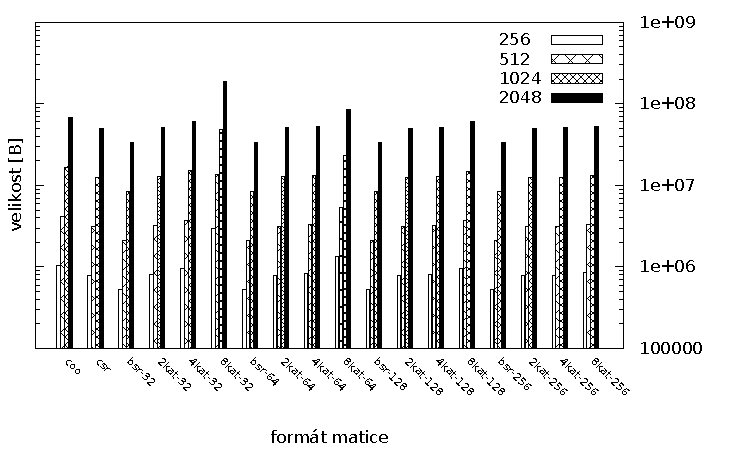
\includegraphics[width=1.0\textwidth]{./images/dense/ram-size}
	\caption{Datová velikost hustých matic v řídkých formátech}
	\label{fig:denram}
\end{figure}

Z měření vyplývá, že se teoretické předpoklady střetly s naměřenými hodnotami. Graf pro násobení matice maticí \ref{fig:denmmm} ukazuje kubickou závislost mezi velikostí matice a časem. Graf pro násobení matice vektorem \ref{fig:denmvm} ukazuje kvadratickou závislost. Velikost datových struktur ukazuje graf \ref{fig:denram}. Lze z něj vyčíst, že COO potřebuje více paměti než CSR, protože ukládá o každém prvku i řádek, kdežto CSR si pro každý řádek pamatuje rozsah prvků a tedy pro každý prvek lze dopočítat, v jakém je řádku. Formát BSR má nejmenší datovou velikost, jelikož bloky ukládá jako husté matice. Formát KAT ukazuje, že uložení stromu sice zvýší celkovou velikost matice, ale ne tak výrazně, aby byl formát nepoužitelný.

Tabulka \ref{overspeed} shrnuje časové a tabulka \ref{overram} paměťové složitosti.

\begin{table}[htb]\label{overspeed}
    \begin{tabular}{r|l|l}
    Formát & Časová složitost MMM    & Časová složitost MVM \\
     \hline
    COO    & jako CSR                                                 & \bigO$(nnz)$                                \\
    CSR    & \bigO($\sum_{i=1}^{n} nnzr_{A,i} \cdot nnzc_{B,i}$) \ref{csrmmm}     & \bigO$(nnz)$                                \\
    BSR    & \bigO($blks \cdot sm\_size^3$)                           & \bigO($blks \cdot sm\_size^2$)              \\
    KAT    & \bigO$(\frac{n^2}{sm\_size} \cdot (height+sm\_size^3)$ & \bigO$(\frac{n^2}{sm\_size} \cdot (height+sm\_size^2)$                                           \\
    \end{tabular} 
    \caption{Přehled časových složitostí násobení matic}
\end{table}


\begin{table}[htb]\label{overram}
    \begin{tabular}{r|l}
    Formát & Paměťová složitost \\
     \hline
    COO    & \bigO($nnz \cdot 3$)                     \\
    CSR    & \bigO($nnz \cdot 2 + m + 1$)               \\
    BSR    & \bigO($blks \cdot sm\_size^2$)                                    \\
    KAT    & \bigO$(k^{height-2}-k-\frac{1}{k} + item\_data)$  \\
    \end{tabular}
    \caption{Přehled paměťových složitostí násobení matic}
\end{table}

\section{Zhodnocení výsledků}

Matice ve formátu BSR dosahovaly velmi špatných výsledků, protože	 jejich bloky jsou pouze husté. V případě větších bloků s menším počtem nulových prvků tak dochází jak k ukládání těchto nulových prvků zbytečně, tak se tím zpomalí výpočet.

Největším zlepšením byla matice KAT pro matici exdata-1 \cite{mtxexdata}, kde se výpočet zrychlil o více než dvojnásobek. Důvodem bylo efektivní rozdělení matice na husté a řídké části. I paměťová velikost byla srovnatelná s formátem CSR.

U matic, kde není nějaký vzor ve formě bloků, například u matice EX6 \cite{mtxex}, byl formát CSR rychlejší ve všech případech. Za  povšimnutí také stojí to, že v základním nastavení programu nebyl v matici KAT zvolen pro tuto matici ani jeden hustý list.

Také ani jeden hustý list nebyl zvolen pro matici human\_gene2 \cite{mtxhuman}. Vzhledem k její hustotě a velikosti ale pro velké CSR bloky 128 a 256 díky časové a prostorové lokalitě \cite{cachelocal} byly výsledky lepší než v obyčejném CSR.

Přestože se s větším $k$ u KAT matic výrazně snížil počet vnitřních uzlů, tak se celková datová velikost matice výrazně zvýšila. Důvodem je velikost uzlu, která obsahuje $k^2$ ukazatelů na syny. 
